\chapter{Wissenschaftlicher Kontext}
\cite{ion} gibt einen Überblick über die derzeitige Forschung an Gitterionentriebwerken. Im Vordergrund der Herausforderungen steht auch die Verwendung alternativer Treibstoffe, vor allem im Blick auf die Kommerzialisierung von LEO-Missionen. Welche Substanzen das kostenintesive Xenon ersetzen können, ist Mittelpunkt aktueller Forschungsprojekte. Im Rahmen des GIESEPP (Gridded Ion Engine Standardised Electric Propulsion Platform) Projekts wurden in \cite{Prop} verschiedene Treibstoffe für die Verwendung mit Gitterionentriebwerken vorgeschlagen. Diese sind in Tabelle \ref{tab:propellants} mit ihren Eigenschaften aufgelistet. Während Iod bereits in Gitterionentriebwerken in-Orbit getestet wurde \cite{Iodine}, sind einige der anderen vorgeschlagenen Treibstoffe noch nicht in der Raumfahrt allgemein oder in RITs erprobt. Die Untersuchung der Ionisiationseigenschaften von Treibstoffen dieser Art ist daher von großer Bedeutung. Es fällt auf, dass die meisten alternativen Treibstoffe unter Standardbedingungen (STP) gasförmig sind, weshalb eine Untersuchung mit einer Anlage wie \textit{ZeroB} sinnvoll ist. Auch besonders interessant ist die Untersuchung von Molekülen, wie Diamantoiden (Adamantan), die eine hohe Dichte und damit ein hohes Masse-zu-Ladungsverhältnis haben. Aufgrund ihres großen Querschnitt, haben sie auch einen hohen Ionisationsquerschnitt \cite{ion}. Diese werden ebenfalls an der JLU untersucht \cite{diamondoids} und sollen in Zukunft auch in \textit{ZeroB} weiter getestet werden. Bisherige Untersuchungen zeigen: Das Problem bei der Verwendung von Diamantoiden ist die Fragmentation der Moleküle in viele kleinere Ionen. Die Ionisationsenergie ist nur geringfügig kleiner als die Energie, die benötigt wird, um das Molekül zu fragmentieren. Durch die Modifikation dieser Moleküle, erhofft man sich eine Verbesserung der Ionisationsqualität. 

Eine weitere Gruppe von Molekülen, die untersucht werden sind aromatische Hydrokarbone, wie Naphthalen. Diese haben ähnliche Massen und Ionisationsenergien wie Diamantoide, weisen aber eine geringe Fragmentation auf. \cite{hydrocarbons} zeigt, dass Moleküle wie Naphthalen einen alternativen Treibstoff darstellen könnten.

Eine massenspektrometrische Anlage, wie \textit{Zero-B}, wird in einigen dieser Arbeiten bereits verwendet. Sie eignet sich besonders gut für die Untersuchung von Molekülen, da die unterschiedlichen Massen der Fragmente ihre Identifikation erlaubt. Die Darstellung der Fragmentationsquerschnitte gegenüber der Ionisationsquerschnitte sind hilfreich, um die Art der Fragmentation zu verstehen und möglicherweise zu verhindern. Eine Optimierung der Anlage, wie sie in dieser Arbeit durchgeführt wird, ist daher von  Bedeutung für die Forschung an alternativen Treibstoffen.

\begin{table}
    \centering
    \renewcommand{\arraystretch}{1.2}
    \caption[Übersicht alternativer Treibstoffe aus \cite{Prop}]{Übersicht alternativer Treibstoffe aus \cite{Prop}. Die meisten Treibstoffe sind unter Standardbedingungen (STP) gasförmig. Aufgelistet sind: Xenon (Xe), Krypton (Kr), Argon (Ar), Neon (Ne),
    Helium (He), Wasserstoff (H2), Iod (I2),
    Buckminster-Fulleren (C60), Adamantan (C10H16),
    Quecksilber (Hg)}
    \vspace{.5cm}
    \begin{tabular}{lcccccc}
        \toprule
        \textbf{Treibstoff} & \textbf{Masse [u]} & \makecell{\textbf{Aggregat-} \\ \textbf{zustand} \\ \textbf{(STP)}} & \makecell{\textbf{1. / 2.} \\ \textbf{Ionisations-} \\ \textbf{energie [eV]}} & \makecell{\textbf{Siede-} \\ \textbf{punkt}} & \makecell{\textbf{Dichte} \\ \textbf{[g/cm$^3$]} \\ \textbf{(STP)}} & \makecell{\textbf{Kosten} \\ \textbf{[\$/100g]}} \\
        \midrule
        Xe   & 131.3  & gasförmig   & 12.13 / 20.97  & 165.1  & 0.0059  & 120  \\
        Kr   & 83.8   & gasförmig   & 14 / 24.36     & 119.7  & 0.0037  & 33   \\
        Ar   & 39.9   & gasförmig   & 15.76 / 27.63  & 87.3   & 0.0018  & 0.5  \\
        Ne   & 20.2   & gasförmig   & 21.56 / 40.96  & 27.1   & 0.0009  & 33   \\
        He   & 4.0    & gasförmig   & 24.59 / 54.41  & 4.2    & 0.0002  & 5.2  \\
        H$_2$   & 2.0    & gasförmig   & 15.43 / -      & 20.3  & 0.00009 & 12   \\
        I$_2$ (I) & 253.8 (126.9) & fest & 9.3 / - & 457.6  & 4.933   & 8.3   \\
        C$_{60}$  & 720.6  & fest & 7.5 / 12      & 823  & 1.65    & 1125  \\
        C$_{10}$H$_{16}$ & 136.2  & fest & 9.23 / -      & 543.18   & 1.07    & 100   \\
        Hg   & 200.6  & flüssig & 10.44 / 18.76  & 629.8    & 13.534  & 48    \\
        \bottomrule
    \end{tabular}

    \label{tab:propellants}
\end{table}

Wie bereits erwähnt, ist eine Untersuchung der Ionisationseigenschaften eines Gases eine komplexe Aufgabe. Straub \textit{et al.} \cite{Straub}\cite{Straub2} haben dennoch bereits 1995 Ionisationsquerschnitte verschiedener Gase und Moleküle experimentell bestimmt. Die Messungen wurden mit einer Anlage (Abb. \ref{fig:Straub}) durchgeführt, die der in dieser Arbeit verwendeten stark ähnelt. Bei der Umsetzung und Validation der \textit{Zero-B}-Anlage wurde auf die Ergebnisse dieser Arbeiten zurückgegriffen. Eine Alternative für die Bestimmung Methode wird in \cite{other_method} beschrieben. Hierbei wird die Ionisation nicht unter Einzelstoßbedingungen untersucht, sondern ein Neutralteilchenstrahl wird mit einem Elektronenstrahl gekreuzt. Die Vorteile die die kontrollierten Rahmenbedingungen der Einzelstoßionisation bieten überwiegen jedoch für die Untersuchung von Treibstoffen, da so mehr Informationen über die Ionisationsprozesse gewonnen werden können.

Stoßionisationsmassenspektrometrie ist seit den 60er Jahren eine etablierte Methode zur Bestimmung von Ionisationsquerschnitten \cite{EITOFMS}. Die Methodik die von Straub \textit{et al.} und in dieser Arbeit verwendet wurde basiert auf dem Delayed Extraction Time-of-Flight (DETOF)-Prinzip. Diese wurde bereits 1955 von Wiley und McLaren zur Verbesserung der Auflösung von Massenspektrometern vorgeschlagen \cite{DETOF} und wird heute noch in optimierter Ausführung in vielen Anlagen verwendet. Die Methode basiert auf der Verzögerung der Ionenextraktion aus der Ionenquelle, um die zeitliche Verteilung der Ionen zu vergrößern. Die Ionen werden dann in einem elektrischen Feld beschleunigt. Durch die Verzögerung der Extraktion, entfernen sich Ionen mit höherer kinetischer Energie weiter von der Extraktionselektrode als langsamere. Bei anschließenden Beschleunigung werden die langsamen Ionen stärker beschleunigt und so kann die Energieverteilung der Ionen kompensiert werden. Die Flugzeit hängt dann stärker von der Masse und Ladung der Teilchen ab. 

\begin{figure}
    \centering
    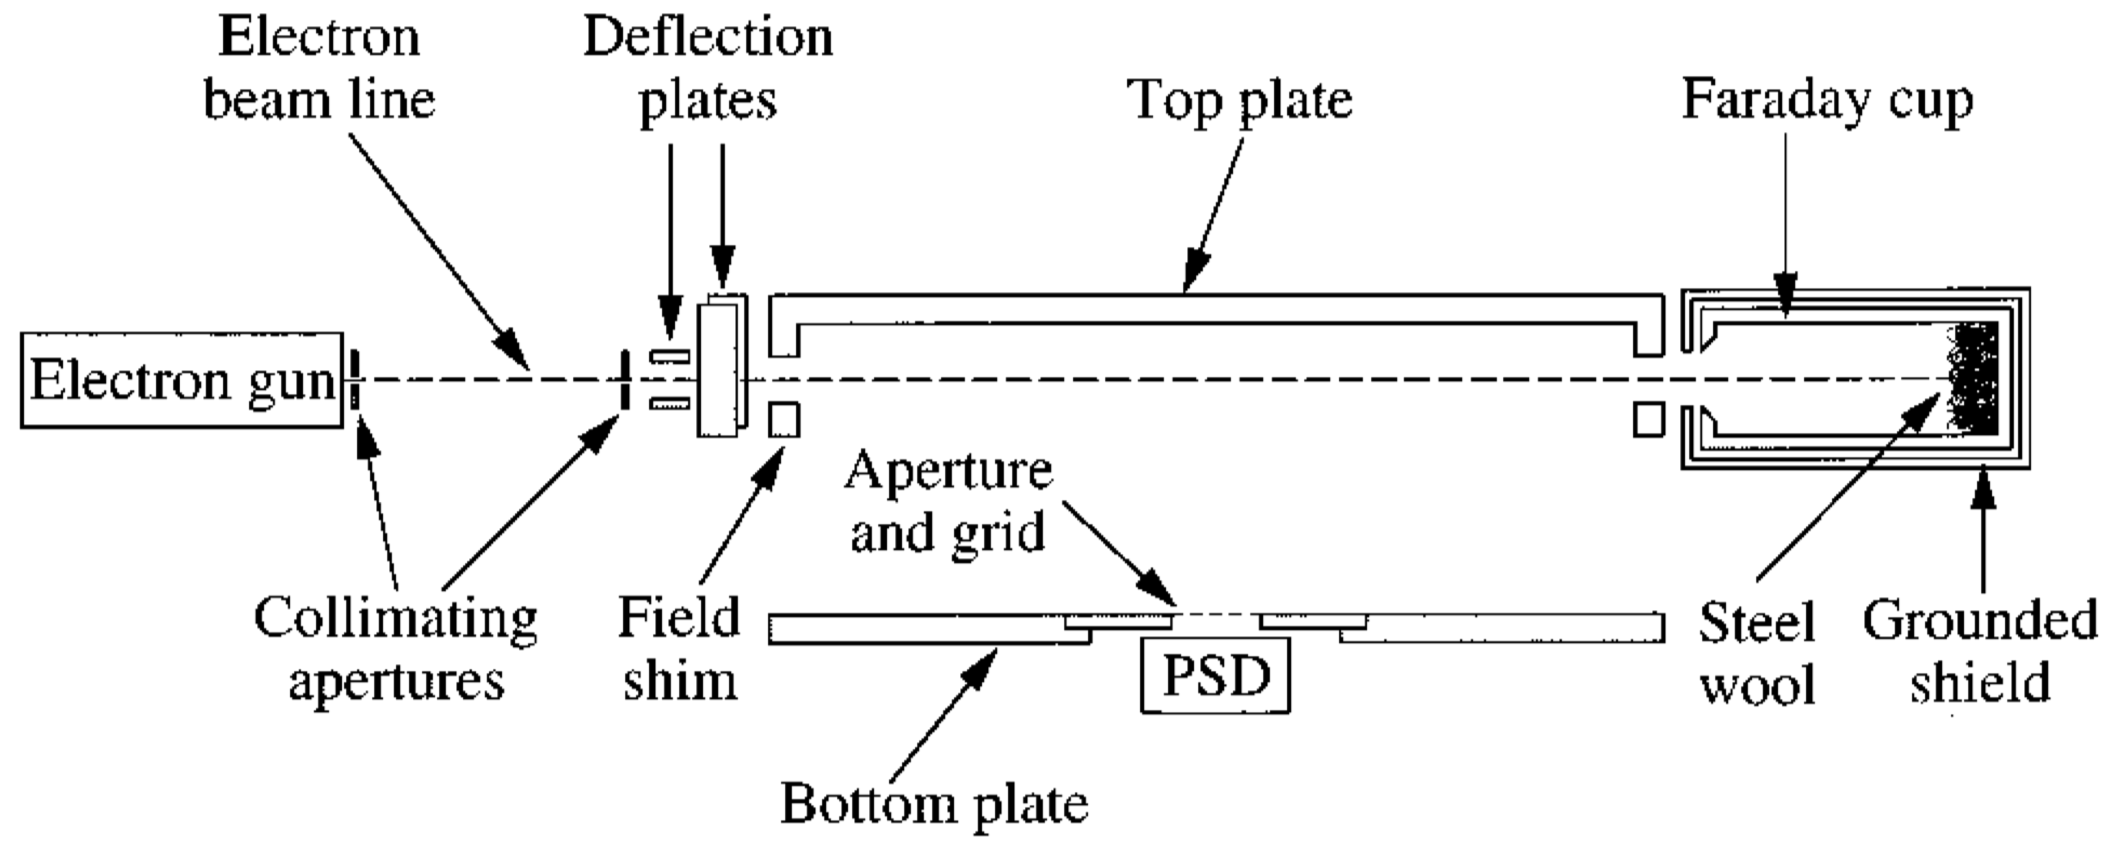
\includegraphics[width=0.9\textwidth]{Straub.png}
    \caption[Anlage zur Messung von Ionisationsquerschnitten aus \cite{Straub2}]{Anlage zur Messung von Ionisationsquerschnitten aus \cite{Straub2}. Der Aufbau ähnelt stark dem der in Kapitel \ref{chap:Aufbau} beschriebenen \textit{Zero-B}-Anlage, mit dem Unterschied, dass die Anlage von Straub eine geringere Flugstrecke zum Detektor hat und auf Linsen verzichtet.}
    \label{fig:Straub}
\end{figure}

Die Untersuchung der Elektronenstoßionisation ist seit vielen Jahren ein zentrales Thema in der Atom- und Plasmaphysik. Für die Analyse sollen in Kapitel \ref{chap:ion} die physikalischen Grundlagen der Elektronenstoßionisation und die Ansätze für theoretische Beschreibungen der verschiedenen Ionisationsprozesse erläutert werden.